% Options for packages loaded elsewhere
\PassOptionsToPackage{unicode}{hyperref}
\PassOptionsToPackage{hyphens}{url}
\PassOptionsToPackage{dvipsnames,svgnames,x11names}{xcolor}
%
\documentclass[
  letterpaper,
  DIV=11,
  numbers=noendperiod]{scrartcl}

\usepackage{amsmath,amssymb}
\usepackage{iftex}
\ifPDFTeX
  \usepackage[T1]{fontenc}
  \usepackage[utf8]{inputenc}
  \usepackage{textcomp} % provide euro and other symbols
\else % if luatex or xetex
  \usepackage{unicode-math}
  \defaultfontfeatures{Scale=MatchLowercase}
  \defaultfontfeatures[\rmfamily]{Ligatures=TeX,Scale=1}
\fi
\usepackage{lmodern}
\ifPDFTeX\else  
    % xetex/luatex font selection
\fi
% Use upquote if available, for straight quotes in verbatim environments
\IfFileExists{upquote.sty}{\usepackage{upquote}}{}
\IfFileExists{microtype.sty}{% use microtype if available
  \usepackage[]{microtype}
  \UseMicrotypeSet[protrusion]{basicmath} % disable protrusion for tt fonts
}{}
\makeatletter
\@ifundefined{KOMAClassName}{% if non-KOMA class
  \IfFileExists{parskip.sty}{%
    \usepackage{parskip}
  }{% else
    \setlength{\parindent}{0pt}
    \setlength{\parskip}{6pt plus 2pt minus 1pt}}
}{% if KOMA class
  \KOMAoptions{parskip=half}}
\makeatother
\usepackage{xcolor}
\setlength{\emergencystretch}{3em} % prevent overfull lines
\setcounter{secnumdepth}{-\maxdimen} % remove section numbering
% Make \paragraph and \subparagraph free-standing
\makeatletter
\ifx\paragraph\undefined\else
  \let\oldparagraph\paragraph
  \renewcommand{\paragraph}{
    \@ifstar
      \xxxParagraphStar
      \xxxParagraphNoStar
  }
  \newcommand{\xxxParagraphStar}[1]{\oldparagraph*{#1}\mbox{}}
  \newcommand{\xxxParagraphNoStar}[1]{\oldparagraph{#1}\mbox{}}
\fi
\ifx\subparagraph\undefined\else
  \let\oldsubparagraph\subparagraph
  \renewcommand{\subparagraph}{
    \@ifstar
      \xxxSubParagraphStar
      \xxxSubParagraphNoStar
  }
  \newcommand{\xxxSubParagraphStar}[1]{\oldsubparagraph*{#1}\mbox{}}
  \newcommand{\xxxSubParagraphNoStar}[1]{\oldsubparagraph{#1}\mbox{}}
\fi
\makeatother

\usepackage{color}
\usepackage{fancyvrb}
\newcommand{\VerbBar}{|}
\newcommand{\VERB}{\Verb[commandchars=\\\{\}]}
\DefineVerbatimEnvironment{Highlighting}{Verbatim}{commandchars=\\\{\}}
% Add ',fontsize=\small' for more characters per line
\usepackage{framed}
\definecolor{shadecolor}{RGB}{241,243,245}
\newenvironment{Shaded}{\begin{snugshade}}{\end{snugshade}}
\newcommand{\AlertTok}[1]{\textcolor[rgb]{0.68,0.00,0.00}{#1}}
\newcommand{\AnnotationTok}[1]{\textcolor[rgb]{0.37,0.37,0.37}{#1}}
\newcommand{\AttributeTok}[1]{\textcolor[rgb]{0.40,0.45,0.13}{#1}}
\newcommand{\BaseNTok}[1]{\textcolor[rgb]{0.68,0.00,0.00}{#1}}
\newcommand{\BuiltInTok}[1]{\textcolor[rgb]{0.00,0.23,0.31}{#1}}
\newcommand{\CharTok}[1]{\textcolor[rgb]{0.13,0.47,0.30}{#1}}
\newcommand{\CommentTok}[1]{\textcolor[rgb]{0.37,0.37,0.37}{#1}}
\newcommand{\CommentVarTok}[1]{\textcolor[rgb]{0.37,0.37,0.37}{\textit{#1}}}
\newcommand{\ConstantTok}[1]{\textcolor[rgb]{0.56,0.35,0.01}{#1}}
\newcommand{\ControlFlowTok}[1]{\textcolor[rgb]{0.00,0.23,0.31}{\textbf{#1}}}
\newcommand{\DataTypeTok}[1]{\textcolor[rgb]{0.68,0.00,0.00}{#1}}
\newcommand{\DecValTok}[1]{\textcolor[rgb]{0.68,0.00,0.00}{#1}}
\newcommand{\DocumentationTok}[1]{\textcolor[rgb]{0.37,0.37,0.37}{\textit{#1}}}
\newcommand{\ErrorTok}[1]{\textcolor[rgb]{0.68,0.00,0.00}{#1}}
\newcommand{\ExtensionTok}[1]{\textcolor[rgb]{0.00,0.23,0.31}{#1}}
\newcommand{\FloatTok}[1]{\textcolor[rgb]{0.68,0.00,0.00}{#1}}
\newcommand{\FunctionTok}[1]{\textcolor[rgb]{0.28,0.35,0.67}{#1}}
\newcommand{\ImportTok}[1]{\textcolor[rgb]{0.00,0.46,0.62}{#1}}
\newcommand{\InformationTok}[1]{\textcolor[rgb]{0.37,0.37,0.37}{#1}}
\newcommand{\KeywordTok}[1]{\textcolor[rgb]{0.00,0.23,0.31}{\textbf{#1}}}
\newcommand{\NormalTok}[1]{\textcolor[rgb]{0.00,0.23,0.31}{#1}}
\newcommand{\OperatorTok}[1]{\textcolor[rgb]{0.37,0.37,0.37}{#1}}
\newcommand{\OtherTok}[1]{\textcolor[rgb]{0.00,0.23,0.31}{#1}}
\newcommand{\PreprocessorTok}[1]{\textcolor[rgb]{0.68,0.00,0.00}{#1}}
\newcommand{\RegionMarkerTok}[1]{\textcolor[rgb]{0.00,0.23,0.31}{#1}}
\newcommand{\SpecialCharTok}[1]{\textcolor[rgb]{0.37,0.37,0.37}{#1}}
\newcommand{\SpecialStringTok}[1]{\textcolor[rgb]{0.13,0.47,0.30}{#1}}
\newcommand{\StringTok}[1]{\textcolor[rgb]{0.13,0.47,0.30}{#1}}
\newcommand{\VariableTok}[1]{\textcolor[rgb]{0.07,0.07,0.07}{#1}}
\newcommand{\VerbatimStringTok}[1]{\textcolor[rgb]{0.13,0.47,0.30}{#1}}
\newcommand{\WarningTok}[1]{\textcolor[rgb]{0.37,0.37,0.37}{\textit{#1}}}

\providecommand{\tightlist}{%
  \setlength{\itemsep}{0pt}\setlength{\parskip}{0pt}}\usepackage{longtable,booktabs,array}
\usepackage{calc} % for calculating minipage widths
% Correct order of tables after \paragraph or \subparagraph
\usepackage{etoolbox}
\makeatletter
\patchcmd\longtable{\par}{\if@noskipsec\mbox{}\fi\par}{}{}
\makeatother
% Allow footnotes in longtable head/foot
\IfFileExists{footnotehyper.sty}{\usepackage{footnotehyper}}{\usepackage{footnote}}
\makesavenoteenv{longtable}
\usepackage{graphicx}
\makeatletter
\newsavebox\pandoc@box
\newcommand*\pandocbounded[1]{% scales image to fit in text height/width
  \sbox\pandoc@box{#1}%
  \Gscale@div\@tempa{\textheight}{\dimexpr\ht\pandoc@box+\dp\pandoc@box\relax}%
  \Gscale@div\@tempb{\linewidth}{\wd\pandoc@box}%
  \ifdim\@tempb\p@<\@tempa\p@\let\@tempa\@tempb\fi% select the smaller of both
  \ifdim\@tempa\p@<\p@\scalebox{\@tempa}{\usebox\pandoc@box}%
  \else\usebox{\pandoc@box}%
  \fi%
}
% Set default figure placement to htbp
\def\fps@figure{htbp}
\makeatother

\usepackage{booktabs}
\usepackage{longtable}
\usepackage{array}
\usepackage{multirow}
\usepackage{wrapfig}
\usepackage{float}
\usepackage{colortbl}
\usepackage{pdflscape}
\usepackage{tabu}
\usepackage{threeparttable}
\usepackage{threeparttablex}
\usepackage[normalem]{ulem}
\usepackage{makecell}
\usepackage{xcolor}
\KOMAoption{captions}{tableheading}
\makeatletter
\@ifpackageloaded{caption}{}{\usepackage{caption}}
\AtBeginDocument{%
\ifdefined\contentsname
  \renewcommand*\contentsname{Table of contents}
\else
  \newcommand\contentsname{Table of contents}
\fi
\ifdefined\listfigurename
  \renewcommand*\listfigurename{List of Figures}
\else
  \newcommand\listfigurename{List of Figures}
\fi
\ifdefined\listtablename
  \renewcommand*\listtablename{List of Tables}
\else
  \newcommand\listtablename{List of Tables}
\fi
\ifdefined\figurename
  \renewcommand*\figurename{Figure}
\else
  \newcommand\figurename{Figure}
\fi
\ifdefined\tablename
  \renewcommand*\tablename{Table}
\else
  \newcommand\tablename{Table}
\fi
}
\@ifpackageloaded{float}{}{\usepackage{float}}
\floatstyle{ruled}
\@ifundefined{c@chapter}{\newfloat{codelisting}{h}{lop}}{\newfloat{codelisting}{h}{lop}[chapter]}
\floatname{codelisting}{Listing}
\newcommand*\listoflistings{\listof{codelisting}{List of Listings}}
\makeatother
\makeatletter
\makeatother
\makeatletter
\@ifpackageloaded{caption}{}{\usepackage{caption}}
\@ifpackageloaded{subcaption}{}{\usepackage{subcaption}}
\makeatother

\usepackage{bookmark}

\IfFileExists{xurl.sty}{\usepackage{xurl}}{} % add URL line breaks if available
\urlstyle{same} % disable monospaced font for URLs
\hypersetup{
  pdftitle={Variable Selection},
  colorlinks=true,
  linkcolor={blue},
  filecolor={Maroon},
  citecolor={Blue},
  urlcolor={Blue},
  pdfcreator={LaTeX via pandoc}}


\title{Variable Selection}
\author{}
\date{}

\begin{document}
\maketitle


\begin{Shaded}
\begin{Highlighting}[]
\FunctionTok{library}\NormalTok{(tidyverse)}
\end{Highlighting}
\end{Shaded}

\begin{verbatim}
-- Attaching core tidyverse packages ------------------------ tidyverse 2.0.0 --
v dplyr     1.1.4     v readr     2.1.5
v forcats   1.0.0     v stringr   1.5.1
v ggplot2   3.5.1     v tibble    3.2.1
v lubridate 1.9.3     v tidyr     1.3.1
v purrr     1.0.2     
-- Conflicts ------------------------------------------ tidyverse_conflicts() --
x dplyr::filter() masks stats::filter()
x dplyr::lag()    masks stats::lag()
i Use the conflicted package (<http://conflicted.r-lib.org/>) to force all conflicts to become errors
\end{verbatim}

\begin{Shaded}
\begin{Highlighting}[]
\FunctionTok{library}\NormalTok{(BAS)        }\CommentTok{\# spike‐and‐slab}
\FunctionTok{library}\NormalTok{(rstanarm)   }\CommentTok{\# horseshoe}
\end{Highlighting}
\end{Shaded}

\begin{verbatim}
Loading required package: Rcpp
This is rstanarm version 2.32.1
- See https://mc-stan.org/rstanarm/articles/priors for changes to default priors!
- Default priors may change, so it's safest to specify priors, even if equivalent to the defaults.
- For execution on a local, multicore CPU with excess RAM we recommend calling
  options(mc.cores = parallel::detectCores())
\end{verbatim}

\begin{Shaded}
\begin{Highlighting}[]
\FunctionTok{library}\NormalTok{(loo)}
\end{Highlighting}
\end{Shaded}

\begin{verbatim}
This is loo version 2.8.0
- Online documentation and vignettes at mc-stan.org/loo
- As of v2.0.0 loo defaults to 1 core but we recommend using as many as possible. Use the 'cores' argument or set options(mc.cores = NUM_CORES) for an entire session. 
\end{verbatim}

\begin{Shaded}
\begin{Highlighting}[]
\FunctionTok{library}\NormalTok{(kableExtra)}
\end{Highlighting}
\end{Shaded}

\begin{verbatim}

Attaching package: 'kableExtra'

The following object is masked from 'package:dplyr':

    group_rows
\end{verbatim}

\begin{Shaded}
\begin{Highlighting}[]
\NormalTok{df }\OtherTok{\textless{}{-}} \FunctionTok{read.csv}\NormalTok{(}\StringTok{"Data/student{-}scores{-}clean.csv"}\NormalTok{) }\SpecialCharTok{|\textgreater{}}
  \FunctionTok{select}\NormalTok{(}\SpecialCharTok{{-}}\NormalTok{id, }\SpecialCharTok{{-}}\NormalTok{first\_name, }\SpecialCharTok{{-}}\NormalTok{last\_name, }\SpecialCharTok{{-}}\NormalTok{email) }\SpecialCharTok{|\textgreater{}}
  \FunctionTok{mutate}\NormalTok{(}
    \AttributeTok{gender                  =} \FunctionTok{factor}\NormalTok{(gender, }\AttributeTok{labels =} \FunctionTok{c}\NormalTok{(}\StringTok{"Female"}\NormalTok{,}\StringTok{"Male"}\NormalTok{)),}
    \AttributeTok{part\_time\_job           =} \FunctionTok{factor}\NormalTok{(part\_time\_job),}
    \AttributeTok{extracurricular\_activities =} \FunctionTok{factor}\NormalTok{(extracurricular\_activities),}
    \AttributeTok{career\_aspiration       =} \FunctionTok{factor}\NormalTok{(career\_aspiration)}
\NormalTok{  )}

\CommentTok{\# keep only non{-}collinear behavioral/demographic predictors}
\NormalTok{vars\_behavioral }\OtherTok{\textless{}{-}} \FunctionTok{c}\NormalTok{(}\StringTok{"gender"}\NormalTok{, }\StringTok{"part\_time\_job"}\NormalTok{, }
                     \StringTok{"absence\_days"}\NormalTok{, }\StringTok{"extracurricular\_activities"}\NormalTok{, }
                     \StringTok{"weekly\_self\_study\_hours"}\NormalTok{, }\StringTok{"career\_aspiration"}\NormalTok{)}

\NormalTok{df\_sub }\OtherTok{\textless{}{-}}\NormalTok{ df }\SpecialCharTok{\%\textgreater{}\%} \FunctionTok{select}\NormalTok{(average\_score, }\FunctionTok{all\_of}\NormalTok{(vars\_behavioral))}
\end{Highlighting}
\end{Shaded}

\begin{Shaded}
\begin{Highlighting}[]
\NormalTok{bas\_fit }\OtherTok{\textless{}{-}} \FunctionTok{bas.lm}\NormalTok{(}
\NormalTok{  average\_score }\SpecialCharTok{\textasciitilde{}}\NormalTok{ ., }
  \AttributeTok{data      =}\NormalTok{ df\_sub, }
  \AttributeTok{prior     =} \StringTok{"ZS{-}null"}\NormalTok{, }
  \AttributeTok{modelprior =} \FunctionTok{uniform}\NormalTok{(),}
  \AttributeTok{n.models  =} \DecValTok{2}\SpecialCharTok{\^{}}\FunctionTok{length}\NormalTok{(vars\_behavioral)}
\NormalTok{)}

\CommentTok{\# posterior inclusion probabilities (PIP)}
\NormalTok{pip }\OtherTok{\textless{}{-}} \FunctionTok{summary}\NormalTok{(bas\_fit)}
\end{Highlighting}
\end{Shaded}

\begin{Shaded}
\begin{Highlighting}[]
\NormalTok{hs\_fit }\OtherTok{\textless{}{-}} \FunctionTok{stan\_glm}\NormalTok{(}
\NormalTok{  average\_score }\SpecialCharTok{\textasciitilde{}}\NormalTok{ ., }
  \AttributeTok{data            =}\NormalTok{ df\_sub, }
  \AttributeTok{family          =} \FunctionTok{gaussian}\NormalTok{(),}
  \AttributeTok{prior\_intercept =} \FunctionTok{normal}\NormalTok{(}\DecValTok{0}\NormalTok{, }\DecValTok{10}\NormalTok{),}
  \AttributeTok{prior           =} \FunctionTok{hs}\NormalTok{(),     }\CommentTok{\# global–local horseshoe}
  \AttributeTok{chains          =} \DecValTok{4}\NormalTok{, }
  \AttributeTok{iter            =} \DecValTok{2000}\NormalTok{,}
  \AttributeTok{seed            =} \DecValTok{2025}
\NormalTok{)}
\end{Highlighting}
\end{Shaded}

\begin{verbatim}

SAMPLING FOR MODEL 'continuous' NOW (CHAIN 1).
Chain 1: 
Chain 1: Gradient evaluation took 0.000186 seconds
Chain 1: 1000 transitions using 10 leapfrog steps per transition would take 1.86 seconds.
Chain 1: Adjust your expectations accordingly!
Chain 1: 
Chain 1: 
Chain 1: Iteration:    1 / 2000 [  0%]  (Warmup)
Chain 1: Iteration:  200 / 2000 [ 10%]  (Warmup)
Chain 1: Iteration:  400 / 2000 [ 20%]  (Warmup)
Chain 1: Iteration:  600 / 2000 [ 30%]  (Warmup)
Chain 1: Iteration:  800 / 2000 [ 40%]  (Warmup)
Chain 1: Iteration: 1000 / 2000 [ 50%]  (Warmup)
Chain 1: Iteration: 1001 / 2000 [ 50%]  (Sampling)
Chain 1: Iteration: 1200 / 2000 [ 60%]  (Sampling)
Chain 1: Iteration: 1400 / 2000 [ 70%]  (Sampling)
Chain 1: Iteration: 1600 / 2000 [ 80%]  (Sampling)
Chain 1: Iteration: 1800 / 2000 [ 90%]  (Sampling)
Chain 1: Iteration: 2000 / 2000 [100%]  (Sampling)
Chain 1: 
Chain 1:  Elapsed Time: 6.253 seconds (Warm-up)
Chain 1:                3.518 seconds (Sampling)
Chain 1:                9.771 seconds (Total)
Chain 1: 

SAMPLING FOR MODEL 'continuous' NOW (CHAIN 2).
Chain 2: 
Chain 2: Gradient evaluation took 1.1e-05 seconds
Chain 2: 1000 transitions using 10 leapfrog steps per transition would take 0.11 seconds.
Chain 2: Adjust your expectations accordingly!
Chain 2: 
Chain 2: 
Chain 2: Iteration:    1 / 2000 [  0%]  (Warmup)
Chain 2: Iteration:  200 / 2000 [ 10%]  (Warmup)
Chain 2: Iteration:  400 / 2000 [ 20%]  (Warmup)
Chain 2: Iteration:  600 / 2000 [ 30%]  (Warmup)
Chain 2: Iteration:  800 / 2000 [ 40%]  (Warmup)
Chain 2: Iteration: 1000 / 2000 [ 50%]  (Warmup)
Chain 2: Iteration: 1001 / 2000 [ 50%]  (Sampling)
Chain 2: Iteration: 1200 / 2000 [ 60%]  (Sampling)
Chain 2: Iteration: 1400 / 2000 [ 70%]  (Sampling)
Chain 2: Iteration: 1600 / 2000 [ 80%]  (Sampling)
Chain 2: Iteration: 1800 / 2000 [ 90%]  (Sampling)
Chain 2: Iteration: 2000 / 2000 [100%]  (Sampling)
Chain 2: 
Chain 2:  Elapsed Time: 7.564 seconds (Warm-up)
Chain 2:                3.588 seconds (Sampling)
Chain 2:                11.152 seconds (Total)
Chain 2: 

SAMPLING FOR MODEL 'continuous' NOW (CHAIN 3).
Chain 3: 
Chain 3: Gradient evaluation took 1.2e-05 seconds
Chain 3: 1000 transitions using 10 leapfrog steps per transition would take 0.12 seconds.
Chain 3: Adjust your expectations accordingly!
Chain 3: 
Chain 3: 
Chain 3: Iteration:    1 / 2000 [  0%]  (Warmup)
Chain 3: Iteration:  200 / 2000 [ 10%]  (Warmup)
Chain 3: Iteration:  400 / 2000 [ 20%]  (Warmup)
Chain 3: Iteration:  600 / 2000 [ 30%]  (Warmup)
Chain 3: Iteration:  800 / 2000 [ 40%]  (Warmup)
Chain 3: Iteration: 1000 / 2000 [ 50%]  (Warmup)
Chain 3: Iteration: 1001 / 2000 [ 50%]  (Sampling)
Chain 3: Iteration: 1200 / 2000 [ 60%]  (Sampling)
Chain 3: Iteration: 1400 / 2000 [ 70%]  (Sampling)
Chain 3: Iteration: 1600 / 2000 [ 80%]  (Sampling)
Chain 3: Iteration: 1800 / 2000 [ 90%]  (Sampling)
Chain 3: Iteration: 2000 / 2000 [100%]  (Sampling)
Chain 3: 
Chain 3:  Elapsed Time: 8.887 seconds (Warm-up)
Chain 3:                7.01 seconds (Sampling)
Chain 3:                15.897 seconds (Total)
Chain 3: 

SAMPLING FOR MODEL 'continuous' NOW (CHAIN 4).
Chain 4: 
Chain 4: Gradient evaluation took 1.4e-05 seconds
Chain 4: 1000 transitions using 10 leapfrog steps per transition would take 0.14 seconds.
Chain 4: Adjust your expectations accordingly!
Chain 4: 
Chain 4: 
Chain 4: Iteration:    1 / 2000 [  0%]  (Warmup)
Chain 4: Iteration:  200 / 2000 [ 10%]  (Warmup)
Chain 4: Iteration:  400 / 2000 [ 20%]  (Warmup)
Chain 4: Iteration:  600 / 2000 [ 30%]  (Warmup)
Chain 4: Iteration:  800 / 2000 [ 40%]  (Warmup)
Chain 4: Iteration: 1000 / 2000 [ 50%]  (Warmup)
Chain 4: Iteration: 1001 / 2000 [ 50%]  (Sampling)
Chain 4: Iteration: 1200 / 2000 [ 60%]  (Sampling)
Chain 4: Iteration: 1400 / 2000 [ 70%]  (Sampling)
Chain 4: Iteration: 1600 / 2000 [ 80%]  (Sampling)
Chain 4: Iteration: 1800 / 2000 [ 90%]  (Sampling)
Chain 4: Iteration: 2000 / 2000 [100%]  (Sampling)
Chain 4: 
Chain 4:  Elapsed Time: 9.966 seconds (Warm-up)
Chain 4:                6.939 seconds (Sampling)
Chain 4:                16.905 seconds (Total)
Chain 4: 
\end{verbatim}

\begin{verbatim}
Warning: There were 21 divergent transitions after warmup. See
https://mc-stan.org/misc/warnings.html#divergent-transitions-after-warmup
to find out why this is a problem and how to eliminate them.
\end{verbatim}

\begin{verbatim}
Warning: Examine the pairs() plot to diagnose sampling problems
\end{verbatim}

\begin{Shaded}
\begin{Highlighting}[]
\FunctionTok{print}\NormalTok{(hs\_fit, }\AttributeTok{digits =} \DecValTok{2}\NormalTok{)}
\end{Highlighting}
\end{Shaded}

\begin{verbatim}
stan_glm
 family:       gaussian [identity]
 formula:      average_score ~ .
 observations: 2000
 predictors:   22
------
                                       Median MAD_SD
(Intercept)                            77.59   0.68 
genderMale                             -0.28   0.24 
part_time_job1                         -0.08   0.25 
absence_days                            0.03   0.05 
extracurricular_activities1            -0.05   0.21 
weekly_self_study_hours                 0.13   0.02 
career_aspirationArtist                 2.62   0.87 
career_aspirationBanker                 1.42   0.64 
career_aspirationBusiness Owner        -3.44   0.69 
career_aspirationConstruction Engineer  3.04   0.78 
career_aspirationDesigner               2.57   0.84 
career_aspirationDoctor                 7.39   0.70 
career_aspirationGame Developer         3.67   0.85 
career_aspirationGovernment Officer     2.00   0.88 
career_aspirationLawyer                 2.69   0.66 
career_aspirationReal Estate Developer  0.99   0.87 
career_aspirationScientist              4.40   0.93 
career_aspirationSoftware Engineer      1.50   0.59 
career_aspirationStock Investor         1.13   0.80 
career_aspirationTeacher                1.04   0.88 
career_aspirationUnknown               -0.03   0.47 
career_aspirationWriter                 3.00   0.97 

Auxiliary parameter(s):
      Median MAD_SD
sigma 4.75   0.08  

------
* For help interpreting the printed output see ?print.stanreg
* For info on the priors used see ?prior_summary.stanreg
\end{verbatim}

\begin{Shaded}
\begin{Highlighting}[]
\FunctionTok{plot}\NormalTok{(hs\_fit, }\AttributeTok{pars =} \FunctionTok{c}\NormalTok{(}\StringTok{"beta"}\NormalTok{), }\AttributeTok{prob =} \FloatTok{0.9}\NormalTok{)}
\end{Highlighting}
\end{Shaded}

\pandocbounded{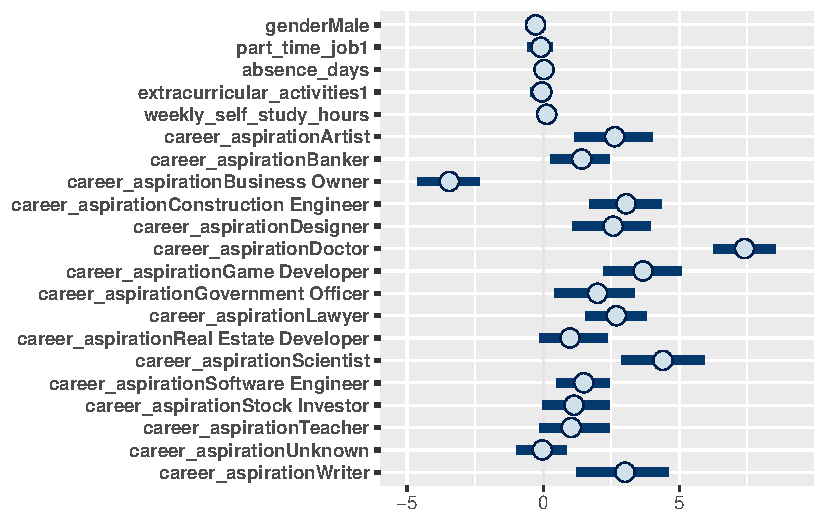
\includegraphics[keepaspectratio]{Bayesian-VS_files/figure-pdf/unnamed-chunk-5-1.pdf}}

\begin{Shaded}
\begin{Highlighting}[]
\NormalTok{loo\_fit }\OtherTok{\textless{}{-}} \FunctionTok{loo}\NormalTok{(hs\_fit)}

\CommentTok{\# extract into a tibble}
\NormalTok{loo\_df }\OtherTok{\textless{}{-}} \FunctionTok{tibble}\NormalTok{(}
  \AttributeTok{Metric        =} \FunctionTok{c}\NormalTok{(}\StringTok{"elpd\_loo"}\NormalTok{, }\StringTok{"se\_elpd\_loo"}\NormalTok{, }\StringTok{"p\_loo"}\NormalTok{),}
  \AttributeTok{Estimate      =} \FunctionTok{c}\NormalTok{(loo\_fit}\SpecialCharTok{$}\NormalTok{estimates[}\StringTok{"elpd\_loo"}\NormalTok{,}\StringTok{"Estimate"}\NormalTok{],}
\NormalTok{                    loo\_fit}\SpecialCharTok{$}\NormalTok{estimates[}\StringTok{"elpd\_loo"}\NormalTok{,}\StringTok{"SE"}\NormalTok{],}
\NormalTok{                    loo\_fit}\SpecialCharTok{$}\NormalTok{estimates[}\StringTok{"p\_loo"}\NormalTok{,}\StringTok{"Estimate"}\NormalTok{])}
\NormalTok{)}

\CommentTok{\# display}
\FunctionTok{kable}\NormalTok{(}
\NormalTok{  loo\_df,}
  \AttributeTok{digits  =} \DecValTok{2}\NormalTok{,}
  \AttributeTok{caption =} \StringTok{"LOO Cross‐Validation Metrics"}
\NormalTok{)}
\end{Highlighting}
\end{Shaded}

\begin{longtable}[]{@{}lr@{}}
\caption{LOO Cross‐Validation Metrics}\tabularnewline
\toprule\noalign{}
Metric & Estimate \\
\midrule\noalign{}
\endfirsthead
\toprule\noalign{}
Metric & Estimate \\
\midrule\noalign{}
\endhead
\bottomrule\noalign{}
\endlastfoot
elpd\_loo & -5965.97 \\
se\_elpd\_loo & 31.85 \\
p\_loo & 22.22 \\
\end{longtable}

\begin{Shaded}
\begin{Highlighting}[]
\NormalTok{df\_sub }\OtherTok{\textless{}{-}}\NormalTok{ df }\SpecialCharTok{\%\textgreater{}\%}
  \FunctionTok{select}\NormalTok{(}
\NormalTok{    average\_score,}
    \SpecialCharTok{{-}}\FunctionTok{starts\_with}\NormalTok{(}\StringTok{"career\_aspiration"}\NormalTok{)}
\NormalTok{  )}
\end{Highlighting}
\end{Shaded}

\[
\begin{aligned}
\text{average_score}_i \;|\;\beta_0, \beta_1, \beta_2, \beta_3, b_{0[\text{aspiration}_i]}, \sigma^2
&\sim \mathcal{N}\bigl(\mu_i,\;\sigma^2\bigr), \\[4pt]
\mu_i &= \beta_0
         + \beta_1\,\text{weekly_self_study_hours}_i
         + \beta_2\,\text{absence_days}_i
         + \beta_3\,\text{extracurricular_activities}_i
         + b_{0[\text{aspiration}_i]}, \\[4pt]
b_{0[j]} &\sim \mathcal{N}(0,\;\tau^2), 
\quad j = 1,\dots,J
\end{aligned}
\]

\begin{Shaded}
\begin{Highlighting}[]
\CommentTok{\# random intercept}
\NormalTok{model1 }\OtherTok{\textless{}{-}} \FunctionTok{stan\_lmer}\NormalTok{(}
\NormalTok{  average\_score }\SpecialCharTok{\textasciitilde{}}\NormalTok{ weekly\_self\_study\_hours }
                \SpecialCharTok{+}\NormalTok{ absence\_days }
                \SpecialCharTok{+}\NormalTok{ extracurricular\_activities }
                \SpecialCharTok{+}\NormalTok{ (}\DecValTok{1} \SpecialCharTok{|}\NormalTok{ career\_aspiration),}
  \AttributeTok{data =}\NormalTok{ df,}
  \AttributeTok{prior\_intercept    =} \FunctionTok{normal}\NormalTok{(}\DecValTok{75}\NormalTok{, }\DecValTok{10}\NormalTok{),}
  \AttributeTok{prior              =} \FunctionTok{normal}\NormalTok{(}\DecValTok{0}\NormalTok{, }\DecValTok{5}\NormalTok{),}
  \AttributeTok{prior\_covariance   =} \FunctionTok{decov}\NormalTok{(}\AttributeTok{regularization =} \DecValTok{2}\NormalTok{),}
  \AttributeTok{chains =} \DecValTok{4}\NormalTok{, }\AttributeTok{iter =} \DecValTok{2000}\NormalTok{, }\AttributeTok{seed =} \DecValTok{123}
\NormalTok{)}
\end{Highlighting}
\end{Shaded}

\begin{verbatim}

SAMPLING FOR MODEL 'continuous' NOW (CHAIN 1).
Chain 1: 
Chain 1: Gradient evaluation took 8.7e-05 seconds
Chain 1: 1000 transitions using 10 leapfrog steps per transition would take 0.87 seconds.
Chain 1: Adjust your expectations accordingly!
Chain 1: 
Chain 1: 
Chain 1: Iteration:    1 / 2000 [  0%]  (Warmup)
Chain 1: Iteration:  200 / 2000 [ 10%]  (Warmup)
Chain 1: Iteration:  400 / 2000 [ 20%]  (Warmup)
Chain 1: Iteration:  600 / 2000 [ 30%]  (Warmup)
Chain 1: Iteration:  800 / 2000 [ 40%]  (Warmup)
Chain 1: Iteration: 1000 / 2000 [ 50%]  (Warmup)
Chain 1: Iteration: 1001 / 2000 [ 50%]  (Sampling)
Chain 1: Iteration: 1200 / 2000 [ 60%]  (Sampling)
Chain 1: Iteration: 1400 / 2000 [ 70%]  (Sampling)
Chain 1: Iteration: 1600 / 2000 [ 80%]  (Sampling)
Chain 1: Iteration: 1800 / 2000 [ 90%]  (Sampling)
Chain 1: Iteration: 2000 / 2000 [100%]  (Sampling)
Chain 1: 
Chain 1:  Elapsed Time: 5.275 seconds (Warm-up)
Chain 1:                1.876 seconds (Sampling)
Chain 1:                7.151 seconds (Total)
Chain 1: 

SAMPLING FOR MODEL 'continuous' NOW (CHAIN 2).
Chain 2: 
Chain 2: Gradient evaluation took 4.9e-05 seconds
Chain 2: 1000 transitions using 10 leapfrog steps per transition would take 0.49 seconds.
Chain 2: Adjust your expectations accordingly!
Chain 2: 
Chain 2: 
Chain 2: Iteration:    1 / 2000 [  0%]  (Warmup)
Chain 2: Iteration:  200 / 2000 [ 10%]  (Warmup)
Chain 2: Iteration:  400 / 2000 [ 20%]  (Warmup)
Chain 2: Iteration:  600 / 2000 [ 30%]  (Warmup)
Chain 2: Iteration:  800 / 2000 [ 40%]  (Warmup)
Chain 2: Iteration: 1000 / 2000 [ 50%]  (Warmup)
Chain 2: Iteration: 1001 / 2000 [ 50%]  (Sampling)
Chain 2: Iteration: 1200 / 2000 [ 60%]  (Sampling)
Chain 2: Iteration: 1400 / 2000 [ 70%]  (Sampling)
Chain 2: Iteration: 1600 / 2000 [ 80%]  (Sampling)
Chain 2: Iteration: 1800 / 2000 [ 90%]  (Sampling)
Chain 2: Iteration: 2000 / 2000 [100%]  (Sampling)
Chain 2: 
Chain 2:  Elapsed Time: 8.142 seconds (Warm-up)
Chain 2:                1.661 seconds (Sampling)
Chain 2:                9.803 seconds (Total)
Chain 2: 

SAMPLING FOR MODEL 'continuous' NOW (CHAIN 3).
Chain 3: 
Chain 3: Gradient evaluation took 5e-05 seconds
Chain 3: 1000 transitions using 10 leapfrog steps per transition would take 0.5 seconds.
Chain 3: Adjust your expectations accordingly!
Chain 3: 
Chain 3: 
Chain 3: Iteration:    1 / 2000 [  0%]  (Warmup)
Chain 3: Iteration:  200 / 2000 [ 10%]  (Warmup)
Chain 3: Iteration:  400 / 2000 [ 20%]  (Warmup)
Chain 3: Iteration:  600 / 2000 [ 30%]  (Warmup)
Chain 3: Iteration:  800 / 2000 [ 40%]  (Warmup)
Chain 3: Iteration: 1000 / 2000 [ 50%]  (Warmup)
Chain 3: Iteration: 1001 / 2000 [ 50%]  (Sampling)
Chain 3: Iteration: 1200 / 2000 [ 60%]  (Sampling)
Chain 3: Iteration: 1400 / 2000 [ 70%]  (Sampling)
Chain 3: Iteration: 1600 / 2000 [ 80%]  (Sampling)
Chain 3: Iteration: 1800 / 2000 [ 90%]  (Sampling)
Chain 3: Iteration: 2000 / 2000 [100%]  (Sampling)
Chain 3: 
Chain 3:  Elapsed Time: 9.511 seconds (Warm-up)
Chain 3:                2.025 seconds (Sampling)
Chain 3:                11.536 seconds (Total)
Chain 3: 

SAMPLING FOR MODEL 'continuous' NOW (CHAIN 4).
Chain 4: 
Chain 4: Gradient evaluation took 5.5e-05 seconds
Chain 4: 1000 transitions using 10 leapfrog steps per transition would take 0.55 seconds.
Chain 4: Adjust your expectations accordingly!
Chain 4: 
Chain 4: 
Chain 4: Iteration:    1 / 2000 [  0%]  (Warmup)
Chain 4: Iteration:  200 / 2000 [ 10%]  (Warmup)
Chain 4: Iteration:  400 / 2000 [ 20%]  (Warmup)
Chain 4: Iteration:  600 / 2000 [ 30%]  (Warmup)
Chain 4: Iteration:  800 / 2000 [ 40%]  (Warmup)
Chain 4: Iteration: 1000 / 2000 [ 50%]  (Warmup)
Chain 4: Iteration: 1001 / 2000 [ 50%]  (Sampling)
Chain 4: Iteration: 1200 / 2000 [ 60%]  (Sampling)
Chain 4: Iteration: 1400 / 2000 [ 70%]  (Sampling)
Chain 4: Iteration: 1600 / 2000 [ 80%]  (Sampling)
Chain 4: Iteration: 1800 / 2000 [ 90%]  (Sampling)
Chain 4: Iteration: 2000 / 2000 [100%]  (Sampling)
Chain 4: 
Chain 4:  Elapsed Time: 4.209 seconds (Warm-up)
Chain 4:                1.741 seconds (Sampling)
Chain 4:                5.95 seconds (Total)
Chain 4: 
\end{verbatim}

\[
\begin{aligned}
\text{average\_score}_i \;|\;\beta_0, \beta_1, \beta_2, \beta_3, \mathbf{b}_{[\text{aspiration}_i]}, \sigma^2
&\sim \mathcal{N}\bigl(\mu_i,\;\sigma^2\bigr), \\[4pt]
\mu_i &= \beta_0
         + \beta_1\,\text{weekly_self_study_hours}_i
         + \beta_2\,\text{absence_days}_i
         + \beta_3\,\text{extracurricular_activities}_i
         + b_{0[\text{aspiration}_i]}
         + b_{1[\text{aspiration}_i]}\,\text{weekly_self_study_hours}_i, \\[4pt]
\begin{pmatrix}
b_{0[j]} \\[2pt]
b_{1[j]}
\end{pmatrix}
&\sim \mathcal{N}\!\Biggl(\!
\begin{pmatrix}0\\0\end{pmatrix},\;
\Sigma\Biggr),
\quad j = 1,\dots,J
\end{aligned}
\]

\begin{Shaded}
\begin{Highlighting}[]
\CommentTok{\# random intercept + slope on study hours}
\NormalTok{model2 }\OtherTok{\textless{}{-}} \FunctionTok{stan\_lmer}\NormalTok{(}
\NormalTok{  average\_score }\SpecialCharTok{\textasciitilde{}}\NormalTok{ weekly\_self\_study\_hours }
                \SpecialCharTok{+}\NormalTok{ absence\_days }
                \SpecialCharTok{+}\NormalTok{ extracurricular\_activities }
                \SpecialCharTok{+}\NormalTok{ (}\DecValTok{1} \SpecialCharTok{+}\NormalTok{ weekly\_self\_study\_hours }\SpecialCharTok{|}\NormalTok{ career\_aspiration),}
  \AttributeTok{data =}\NormalTok{ df,}
  \AttributeTok{prior\_intercept    =} \FunctionTok{normal}\NormalTok{(}\DecValTok{75}\NormalTok{, }\DecValTok{10}\NormalTok{),}
  \AttributeTok{prior              =} \FunctionTok{normal}\NormalTok{(}\DecValTok{0}\NormalTok{, }\DecValTok{5}\NormalTok{),}
  \AttributeTok{prior\_covariance   =} \FunctionTok{decov}\NormalTok{(}\AttributeTok{regularization =} \DecValTok{2}\NormalTok{),}
  \AttributeTok{chains =} \DecValTok{4}\NormalTok{, }\AttributeTok{iter =} \DecValTok{2000}\NormalTok{, }\AttributeTok{seed =} \DecValTok{123}
\NormalTok{)}
\end{Highlighting}
\end{Shaded}

\begin{verbatim}

SAMPLING FOR MODEL 'continuous' NOW (CHAIN 1).
Chain 1: 
Chain 1: Gradient evaluation took 0.000106 seconds
Chain 1: 1000 transitions using 10 leapfrog steps per transition would take 1.06 seconds.
Chain 1: Adjust your expectations accordingly!
Chain 1: 
Chain 1: 
Chain 1: Iteration:    1 / 2000 [  0%]  (Warmup)
Chain 1: Iteration:  200 / 2000 [ 10%]  (Warmup)
Chain 1: Iteration:  400 / 2000 [ 20%]  (Warmup)
Chain 1: Iteration:  600 / 2000 [ 30%]  (Warmup)
Chain 1: Iteration:  800 / 2000 [ 40%]  (Warmup)
Chain 1: Iteration: 1000 / 2000 [ 50%]  (Warmup)
Chain 1: Iteration: 1001 / 2000 [ 50%]  (Sampling)
Chain 1: Iteration: 1200 / 2000 [ 60%]  (Sampling)
Chain 1: Iteration: 1400 / 2000 [ 70%]  (Sampling)
Chain 1: Iteration: 1600 / 2000 [ 80%]  (Sampling)
Chain 1: Iteration: 1800 / 2000 [ 90%]  (Sampling)
Chain 1: Iteration: 2000 / 2000 [100%]  (Sampling)
Chain 1: 
Chain 1:  Elapsed Time: 24.392 seconds (Warm-up)
Chain 1:                5.982 seconds (Sampling)
Chain 1:                30.374 seconds (Total)
Chain 1: 

SAMPLING FOR MODEL 'continuous' NOW (CHAIN 2).
Chain 2: 
Chain 2: Gradient evaluation took 7.2e-05 seconds
Chain 2: 1000 transitions using 10 leapfrog steps per transition would take 0.72 seconds.
Chain 2: Adjust your expectations accordingly!
Chain 2: 
Chain 2: 
Chain 2: Iteration:    1 / 2000 [  0%]  (Warmup)
Chain 2: Iteration:  200 / 2000 [ 10%]  (Warmup)
Chain 2: Iteration:  400 / 2000 [ 20%]  (Warmup)
Chain 2: Iteration:  600 / 2000 [ 30%]  (Warmup)
Chain 2: Iteration:  800 / 2000 [ 40%]  (Warmup)
Chain 2: Iteration: 1000 / 2000 [ 50%]  (Warmup)
Chain 2: Iteration: 1001 / 2000 [ 50%]  (Sampling)
Chain 2: Iteration: 1200 / 2000 [ 60%]  (Sampling)
Chain 2: Iteration: 1400 / 2000 [ 70%]  (Sampling)
Chain 2: Iteration: 1600 / 2000 [ 80%]  (Sampling)
Chain 2: Iteration: 1800 / 2000 [ 90%]  (Sampling)
Chain 2: Iteration: 2000 / 2000 [100%]  (Sampling)
Chain 2: 
Chain 2:  Elapsed Time: 22.264 seconds (Warm-up)
Chain 2:                7.996 seconds (Sampling)
Chain 2:                30.26 seconds (Total)
Chain 2: 

SAMPLING FOR MODEL 'continuous' NOW (CHAIN 3).
Chain 3: 
Chain 3: Gradient evaluation took 7e-05 seconds
Chain 3: 1000 transitions using 10 leapfrog steps per transition would take 0.7 seconds.
Chain 3: Adjust your expectations accordingly!
Chain 3: 
Chain 3: 
Chain 3: Iteration:    1 / 2000 [  0%]  (Warmup)
Chain 3: Iteration:  200 / 2000 [ 10%]  (Warmup)
Chain 3: Iteration:  400 / 2000 [ 20%]  (Warmup)
Chain 3: Iteration:  600 / 2000 [ 30%]  (Warmup)
Chain 3: Iteration:  800 / 2000 [ 40%]  (Warmup)
Chain 3: Iteration: 1000 / 2000 [ 50%]  (Warmup)
Chain 3: Iteration: 1001 / 2000 [ 50%]  (Sampling)
Chain 3: Iteration: 1200 / 2000 [ 60%]  (Sampling)
Chain 3: Iteration: 1400 / 2000 [ 70%]  (Sampling)
Chain 3: Iteration: 1600 / 2000 [ 80%]  (Sampling)
Chain 3: Iteration: 1800 / 2000 [ 90%]  (Sampling)
Chain 3: Iteration: 2000 / 2000 [100%]  (Sampling)
Chain 3: 
Chain 3:  Elapsed Time: 22.495 seconds (Warm-up)
Chain 3:                6.815 seconds (Sampling)
Chain 3:                29.31 seconds (Total)
Chain 3: 

SAMPLING FOR MODEL 'continuous' NOW (CHAIN 4).
Chain 4: 
Chain 4: Gradient evaluation took 7e-05 seconds
Chain 4: 1000 transitions using 10 leapfrog steps per transition would take 0.7 seconds.
Chain 4: Adjust your expectations accordingly!
Chain 4: 
Chain 4: 
Chain 4: Iteration:    1 / 2000 [  0%]  (Warmup)
Chain 4: Iteration:  200 / 2000 [ 10%]  (Warmup)
Chain 4: Iteration:  400 / 2000 [ 20%]  (Warmup)
Chain 4: Iteration:  600 / 2000 [ 30%]  (Warmup)
Chain 4: Iteration:  800 / 2000 [ 40%]  (Warmup)
Chain 4: Iteration: 1000 / 2000 [ 50%]  (Warmup)
Chain 4: Iteration: 1001 / 2000 [ 50%]  (Sampling)
Chain 4: Iteration: 1200 / 2000 [ 60%]  (Sampling)
Chain 4: Iteration: 1400 / 2000 [ 70%]  (Sampling)
Chain 4: Iteration: 1600 / 2000 [ 80%]  (Sampling)
Chain 4: Iteration: 1800 / 2000 [ 90%]  (Sampling)
Chain 4: Iteration: 2000 / 2000 [100%]  (Sampling)
Chain 4: 
Chain 4:  Elapsed Time: 20.325 seconds (Warm-up)
Chain 4:                7.938 seconds (Sampling)
Chain 4:                28.263 seconds (Total)
Chain 4: 
\end{verbatim}

\begin{Shaded}
\begin{Highlighting}[]
\FunctionTok{print}\NormalTok{(model1, }\AttributeTok{digits =} \DecValTok{2}\NormalTok{)}
\end{Highlighting}
\end{Shaded}

\begin{verbatim}
stan_lmer
 family:       gaussian [identity]
 formula:      average_score ~ weekly_self_study_hours + absence_days + extracurricular_activities + 
       (1 | career_aspiration)
 observations: 2000
------
                            Median MAD_SD
(Intercept)                 79.18   0.68 
weekly_self_study_hours      0.14   0.02 
absence_days                 0.05   0.05 
extracurricular_activities1 -0.09   0.27 

Auxiliary parameter(s):
      Median MAD_SD
sigma 4.74   0.08  

Error terms:
 Groups            Name        Std.Dev.
 career_aspiration (Intercept) 2.56    
 Residual                      4.74    
Num. levels: career_aspiration 17 

------
* For help interpreting the printed output see ?print.stanreg
* For info on the priors used see ?prior_summary.stanreg
\end{verbatim}

\begin{Shaded}
\begin{Highlighting}[]
\FunctionTok{print}\NormalTok{(model2, }\AttributeTok{digits =} \DecValTok{2}\NormalTok{)}
\end{Highlighting}
\end{Shaded}

\begin{verbatim}
stan_lmer
 family:       gaussian [identity]
 formula:      average_score ~ weekly_self_study_hours + absence_days + extracurricular_activities + 
       (1 + weekly_self_study_hours | career_aspiration)
 observations: 2000
------
                            Median MAD_SD
(Intercept)                 79.03   0.58 
weekly_self_study_hours      0.14   0.03 
absence_days                 0.04   0.05 
extracurricular_activities1 -0.09   0.27 

Auxiliary parameter(s):
      Median MAD_SD
sigma 4.72   0.07  

Error terms:
 Groups            Name                    Std.Dev. Corr
 career_aspiration (Intercept)             1.9058       
                   weekly_self_study_hours 0.0912   0.11
 Residual                                  4.7212       
Num. levels: career_aspiration 17 

------
* For help interpreting the printed output see ?print.stanreg
* For info on the priors used see ?prior_summary.stanreg
\end{verbatim}

\begin{Shaded}
\begin{Highlighting}[]
\CommentTok{\#Posterior predictive checks}
\FunctionTok{pp\_check}\NormalTok{(model1)}
\end{Highlighting}
\end{Shaded}

\pandocbounded{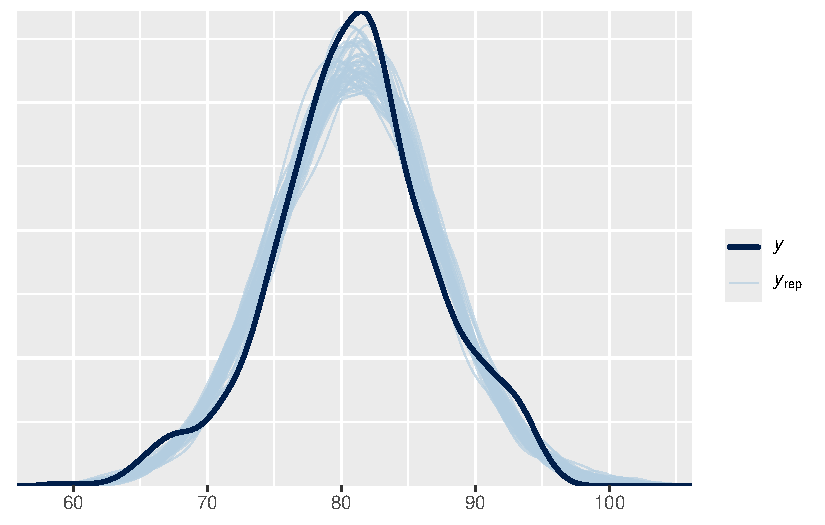
\includegraphics[keepaspectratio]{Bayesian-VS_files/figure-pdf/unnamed-chunk-10-1.pdf}}

\begin{Shaded}
\begin{Highlighting}[]
\FunctionTok{pp\_check}\NormalTok{(model2)}
\end{Highlighting}
\end{Shaded}

\pandocbounded{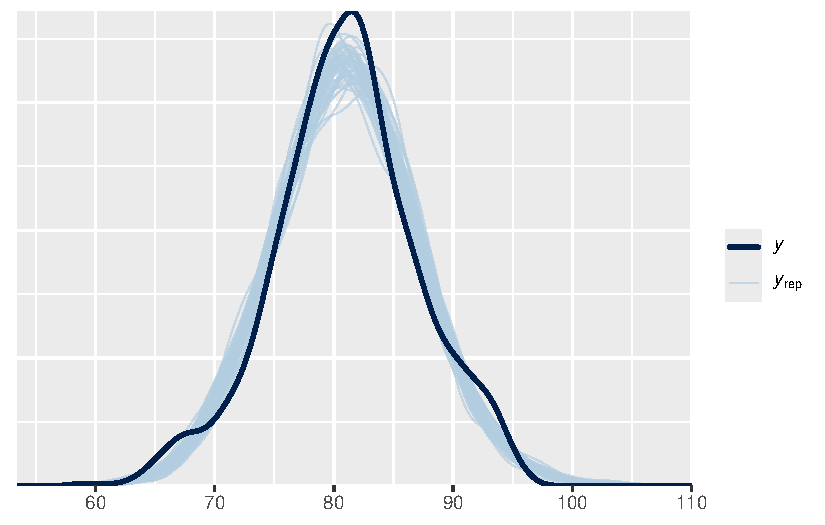
\includegraphics[keepaspectratio]{Bayesian-VS_files/figure-pdf/unnamed-chunk-10-2.pdf}}

\begin{Shaded}
\begin{Highlighting}[]
\CommentTok{\# Compare with LOO}
\NormalTok{loo1 }\OtherTok{\textless{}{-}} \FunctionTok{loo}\NormalTok{(model1)}
\NormalTok{loo2 }\OtherTok{\textless{}{-}} \FunctionTok{loo}\NormalTok{(model2)}
\FunctionTok{loo\_compare}\NormalTok{(loo1, loo2)}
\end{Highlighting}
\end{Shaded}

\begin{verbatim}
       elpd_diff se_diff
model2  0.0       0.0   
model1 -4.9       2.9   
\end{verbatim}




\end{document}
